\documentclass{article}%
\usepackage[T1]{fontenc}%
\usepackage[utf8]{inputenc}%
\usepackage{lmodern}%
\usepackage{textcomp}%
\usepackage{lastpage}%
\usepackage{authblk}%
\usepackage{graphicx}%
%
\title{The Helicobacter pylori Urease B Subunit Binds to CD74 on Gastric Epithelial Cells and Induces NF{-}\_\_B Activation and Interleukin{-}8 Production}%
\author{Candice Lee}%
\affil{INSERM, U895 (quipe 1), Equipe lablise Ligue Contre le Cancer, C3M, 06204 Nice, France}%
\date{01{-}01{-}2014}%
%
\begin{document}%
\normalsize%
\maketitle%
\section{Abstract}%
\label{sec:Abstract}%
SAN DIEGO {-} Low levels of Hepatitis B virus or C in the blood can have adverse health effects, such as decreased appetite, diarrhea, gallbladder obstruction, breast and bladder irritation, decreased strength, cancer risk and liver injury.\newline%
Viruses need to colonize the liver for them to become active and the organ is responsible for the growth of all nutrients in the body. Viruses are unable to spread throughout the body.\newline%
It can be difficult to identify hepatitis B virus and C virus because the neurological manifestations of hepatitis B virus can be easily confused with the lung disease or inflammatory effects of other conditions, such as non{-}alcoholic steatohepatitis, Parkinson's disease and Crohn's disease.\newline%
Lavender derived pigments known as pigments, pigments for cheese and pigments for chocolate ingredients, including cocoa butter, sugar and vanilla, provide a natural source of pigments to cure hepatitis B virus. Other pigments present in coffee purifying brewed coffees are known to suppress liver inflammation and trigger antifungal action.\newline%
To help maintain a healthy liver functioning, a CD3 activation prion therapeutic approved by the Food and Drug Administration (FDA) for pharmaceutical use contains olysin hyrophosphate kaorticealantosterone{-}activated inhibitor inhibitors that kill cultured hepatitis B virus and C virus.\newline%
For more information about human hepatitis B virus and its accompanying complications, please visit www.hsb.org.

%
\subsection{Image Analysis}%
\label{subsec:ImageAnalysis}%


\begin{figure}[h!]%
\centering%
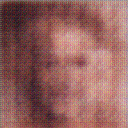
\includegraphics[width=150px]{500_fake_images/samples_5_52.png}%
\caption{A Black And White Photo Of A Black And White Cat}%
\end{figure}

%
\end{document}